\section{Analysis}
\label{sec:Analysis}

The recorded data ist shown in \autoref{tab:Data}. The measured resistance of the thermometers is converted to temperatures using \autoref{eqn:R_T}.
To calculate the energy $E$ added in the observed time interval $\symup{\Delta}t$, the current $I$ ist multiplied with both the length of the time 
interval~$\symup{\Delta}t$ and the applied voltage $U$
\begin{equation}
  E = I \cdot \symup{\Delta}t \cdot U.
  \label{eq:added_E}
\end{equation}

\subsection{Heat capacity at constant pressure}
\label{subsec:Heat capacity at constant volume}
A calculation of the values for $C_\mathrm{p}$ can be done via \autoref{eq:Cp} resulting in

\begin{equation}
  C_\mathrm{p} = \frac{M}{m} \frac{E}{\symup{\Delta}T},
  \label{eq:C_P_calc}
\end{equation}
where $M=\qty{63.546}{\gram\per\mol}$ is the molar mass of Copper and $m=\qty{342}{\gram}$ ist the mass of the copper sample used in the
experiment. 

All the calculated data is also shown in the \autoref{tab:Data}.

\begin{table}
  \centering
  \caption{Measured and calulated data used to determine the heat capacity of Copper. The temperatures are calculated using \autoref{eqn:R_T}, the added %
  energy is received via \autoref{eq:added_E} and for the values of $C_\mathrm{p}$ \autoref{eq:C_P_calc} is used.}
  \label{tab:Data}
  \begin{tabular}{S S S S | S S S | S}
    \toprule
    \multicolumn{4}{c|}{Measured data} & \multicolumn{4}{c}{Calculated data}\\
    {$\symup{\Delta}t \mathbin{/} \unit{s}$} & {$R \mathbin{/} \unit{\ohm}$} & {$I \mathbin{/} \unit{\milli\ampere}$} & {$U \mathbin{/} \unit{V}$} &%
    {$E \mathbin{/} \unit{\joule}$} & {$T \mathbin{/} \unit{\kelvin}$} & {$T \mathbin{/} \unit{\celsius}$} & %
    {$C_\mathrm{p} \mathbin{/} \frac{\unit{\joule}}{\unit{\mol\kelvin}}$}\\
    \midrule
    %200 &  24.4 &  158.5  & 16.63 & 527.2	 & 86  & -186 \\ 
    {-} &  24.4 &  158.5  & 16.63 &  {-}   & 86  & -186 & {-}   \\
    235 &  27.0 &  160.8  & 16.85 & 636.7	 & 93  & -180 & 19.24 \\
    335 &  31.3 &  160.0  & 16.80 & 900.5	 & 103 & -169 & 16.39 \\
    385 &  35.5 &  159.3  & 16.75 & 1027.3 & 113 & -159 & 19.05 \\
    405 &  39.7 &  159.8  & 16.80 & 1087.3 & 123 & -149 & 20.07 \\
    380 &  43.8 &  160.1  & 16.87 & 1026.3 & 133 & -139 & 19.32 \\
    405 &  47.9 &  160.3  & 16.91 & 1097.8 & 143 & -129 & 20.57 \\
    345 &  52.0 &  160.6  & 16.95 & 939.1	 & 153 & -120 & 17.52 \\
    435 &  56.1 &  160.8  & 16.97 & 1187.0 & 163 & -109 & 22.04 \\
    405 &  60.2 &  160.9  & 16.99 & 1107.1 & 173 & -99  & 20.46 \\
    425 &  64.3 &  161.1  & 17.01 & 1164.6 & 183 & -89  & 21.43 \\
    455 &  68.3 &  161.2  & 17.03 & 1249.1 & 193 & -79  & 23.46 \\
    440 &  72.3 &  161.2  & 17.03 & 1207.9 & 203 & -70  & 22.58 \\
    430 &  76.3 &  161.3  & 17.03 & 1181.2 & 213 & -60  & 21.99 \\
    460 &  80.3 &  161.4  & 17.04 & 1265.1 & 223 & -50  & 23.45 \\
    480 &  84.2 &  161.4  & 17.04 & 1320.1 & 232 & -40  & 24.99 \\
    405 &  88.2 &  161.5  & 17.04 & 1114.5 & 243 & -30  & 20.49 \\
    425 &  92.1 &  161.5  & 17.04 & 1169.6 & 252 & -20  & 21.96 \\
    465 &  96.1 &  161.5  & 17.04 & 1279.7 & 263 & -9   & 23.33 \\
    435 & 100.0 &  161.6  & 17.04 & 1197.8 & 273 & 0    & 22.30 \\
    480 & 103.9 &  161.6  & 17.03 & 1321.0 & 283 & 9    & 24.50 \\
    465 & 107.8 &  161.6  & 17.03 & 1279.7 & 293 & 20   & 23.63 \\
    470 & 111.7 &  161.7  & 17.03 & 1294.3 & 303 & 30   & 23.81 \\
    \bottomrule
  \end{tabular}
\end{table}

\subsection{Heat capacity at constant volume}
The heat capacity at constant volume $C_\mathrm{V}$ can be derived by using \autoref{eqn:Cp_CV} and the in \autoref{subsec:Heat capacity at constant volume}
calculated heat capacity at constant pressure. The equation is rearranged to
\begin{equation*}
  C_\mathrm{V} = C_\mathrm{p} - 9 T V_0 \alpha^2 B.
\end{equation*}
The values for the bulk module $B$ and the molar volume $V_0$ can be found in the literature where as the values for the volumetric expansion $\alpha$ is given
in \autoref{fig:alpha}. Hence the measured temperatures are not listed directly in the table an estimation for the volumetric expansion coefficient is performed
via
\begin{equation}
  \alpha (T) = \frac{\alpha_{\symup{i}}-\alpha_{\symup{i-1}}} {T_{\symup{i}}-T_{\symup{i-1}}} (T-T_{\symup{i-1}}) + \alpha_{\symup{i-1}}.
  \label{eq:alpha}
\end{equation}

\begin{figure}
  \centering
  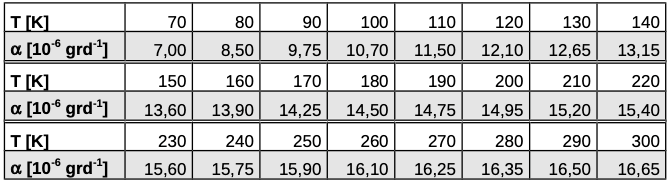
\includegraphics[width = 0.95\textwidth]{content/pics/alpha.png}
  \caption{Values for the volumetric expansion coefficent $\alpha$ of copper. These values and \autoref{eq:alpha} are used to calculate a specific %
  value for each individuel temperature $T$ \cite{V47}.}
  \label{fig:alpha}
\end{figure}

The used values for the bulk module are 
\begin{align*}
  B &= \qty{140e9}{\pascal} \\
  V_0 = \frac{M}{\rho} &= \qty{7.092e-6}{\cubic\metre\per\mol} \\
\end{align*}

In \autoref{tab:C_P,C_V} the values for the molar heat capacity with constant pressure and constant volume are given as well as the used volumetric expansion
coefficent.

\begin{table}
  \centering
  \caption{Calculated values for the volumetric expansion coefficient $\alpha$ and the heat capacity for constant pressure $C_{\symup{p}}$ and constant %
  volume $C_{\symup{V}}$.}
  \label{tab:C_P,C_V}
  \begin{tabular}{S S S S}
    \toprule
    {$T \mathbin{/} \unit{\kelvin}$} & {$\alpha \mathbin{/} 10^{-6}\,\frac{1}{\unit{\kelvin}}$} & {$C_{\symup{p}} \mathbin{/} \frac{\unit{\joule}}{\unit{\mol\kelvin}}$} & %
    {$C_{\symup{V}} \mathbin{/} \frac{\unit{\joule}}{\unit{\mol\kelvin}}$} \\
    \midrule
    %86  & 9.37  & 0.00  & -0.07 \\
    93  & 10.04 & 19.24 & 19.16 \\
    103 & 10.96 & 16.39 & 16.28 \\
    113 & 11.70 & 19.05 & 18.91 \\
    123 & 12.29 & 20.07 & 19.90 \\
    133 & 12.81 & 19.32 & 19.12 \\
    143 & 13.29 & 20.57 & 20.34 \\
    153 & 13.69 & 17.52 & 17.26 \\
    163 & 14.01 & 22.04 & 21.75 \\
    173 & 14.33 & 20.46 & 20.15 \\
    183 & 14.58 & 21.43 & 21.08 \\
    193 & 14.81 & 23.46 & 23.08 \\
    203 & 15.03 & 22.58 & 22.17 \\
    213 & 15.26 & 21.99 & 21.55 \\
    223 & 15.46 & 23.45 & 22.98 \\
    232 & 15.64 & 24.99 & 24.48 \\
    243 & 15.80 & 20.49 & 19.95 \\
    252 & 15.96 & 21.96 & 21.38 \\
    263 & 16.15 & 23.33 & 22.71 \\
    273 & 16.28 & 22.30 & 21.66 \\
    283 & 16.40 & 24.50 & 23.82 \\
    293 & 16.55 & 23.63 & 22.92 \\
    303 & 16.70 & 23.81 & 23.05 \\
    \bottomrule
  \end{tabular}
\end{table}

\begin{figure}
  \centering
  \includegraphics[width = 0.95\textwidth]{build/C.pdf}
  \caption{Plot of the heat capacity for constant pressure~$C_{\symup{p}}$ and constant Volume~$C_{\symup{V}}$.}
  \label{fig:plot}
\end{figure}

\subsection{The Debye temperature of copper}
\label{subsec:The Debye temperature of copper}
Calculating the Debye temperature $\theta_{\symup{D}}$ can be achieved by looking up values for $\frac{\theta_{\symup{D}}}{T}$ in \autoref{fig:debyetemp} and multiplying
with the temperature $T$. Only values for a temperature of less than $\qty{170}{\kelvin}$ must be looked at. The results are presented in \autoref{tab:debyetemp}.

\begin{table}
  \centering
  \caption{Calculation of the Debye temperature $\theta_{\symup{D}}$ using the values for the heat capacity $C_{\symup{V}}$ and the corresponding values %
  for $\frac{\theta_{\symup{D}}}{T}$ looked up at \autoref{fig:debyetemp}.}
  \label{tab:debyetemp}
  \begin{tabular}{S S S S}
    \toprule
    {$T \mathbin{/} \unit{\kelvin}$} & {$C_{\symup{V}} \mathbin{/} \frac{\unit{\joule}}{\unit{\mol\kelvin}}$} & %
    {$\frac{\theta_{\symup{D}}}{T}$} & {$\theta_{\symup{D}} \mathbin{/} \unit{\kelvin}$} \\
    \midrule
    93  & 19.16 & 2.4 & 223.44 \\
    103 & 16.28 & 3.1 & 320.25 \\
    113 & 18.91 & 2.4 & 271.98 \\
    123 & 19.90 & 2.2 & 271.46 \\
    133 & 19.12 & 2.4 & 319.84 \\
    143 & 20.34 & 2.1 & 300.68 \\
    153 & 17.26 & 2.8 & 428.81 \\
    163 & 21.75 & 1.7 & 277.36 \\
    \midrule
    \midrule
    \multicolumn{3}{l}{\textbf{Mean}} & {$\num{301.73 +- 56.29}$} \\
    \bottomrule
  \end{tabular}
\end{table}

\begin{figure}
  \centering
  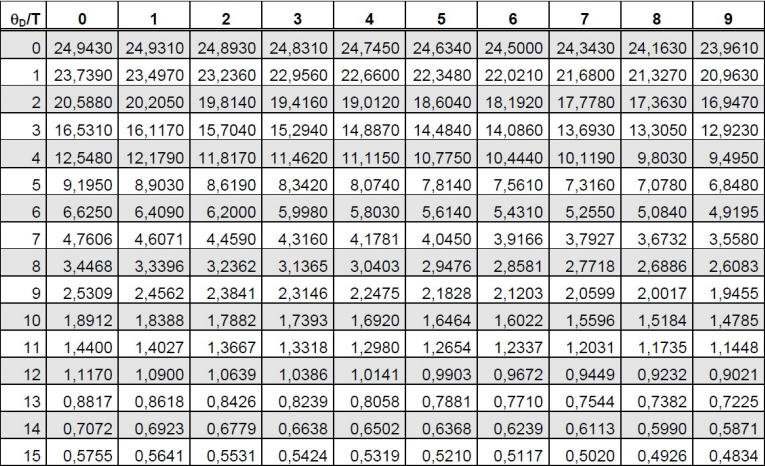
\includegraphics[width = 0.95\textwidth]{content/pics/debyetemp.png}
  \caption{Table used to calulate the Debye temperature. To get a value for $\frac{\theta_{\symup{D}}}{T}$ for a heat capacity $C_{\symup{V}}$ a quantity close %
  to the calculated heat capacity $C_{\symup{V}}$ needs to be found in the table. The left column is the first digit, the top line is the first decimal digit \cite{V47}.} 
  \label{fig:debyetemp}
\end{figure}

\subsection{Calculation of the theoretical Debye frequency and Debye temperature}
\label{subsec:Calculation of the theoretical Debye frequency and Debye temperature}
Using the equation for the density of states function
\begin{equation*}
  Z(\omega)\symup{d}\omega = \frac{V}{2\symup{\pi}^2}\omega^2\left(\frac{1}{v^3_{\text{long}}}+\frac{2}{v^3_{\text{trans}}}\right)
\end{equation*}
the Debye frequency can be calculated as
\begin{equation*}
  \omega = \left(\frac{18\symup{\pi}^2N_{\symup{A}}}{V_0}\left(\frac{1}{v^3_{\text{long}}}+\frac{2}{v^3_{\text{trans}}}\right)^{-1}\right)^{\frac{1}{3}}.
\end{equation*}
Utilizing the Avogadro constant $N_{\symup{A}}$ and the values for the longitudinal and transversal phase velocity 
$v_{\text{long}} = \qty{4.7}{\kilo\metre\per\second}$ and $v_{\text{trans}}=\qty{2.26}{\kilo\metre\per\second}$ as well as the molar volume of the sample $V_0$ the Debye frequency is calculated as
\begin{equation*}
  \omega_{\symup{D}} = \qty{4.35e13}{\per\second}.
\end{equation*}
With the help of the relation
\begin{equation*}
  \theta_{\symup{D}} = \frac{\hbar\omega_{\symup{D}}}{k_{\symup{B}}}
\end{equation*}
the theoretical value for the Debye temperature of copper results as
\begin{equation*}
  \theta_{\symup{D}} = \qty{332.18}{\kelvin}.
\end{equation*}